\documentclass[12pt]{report}
\title{Mid Term Project}
\usepackage{amsmath}
%\usepackage{apacite}
\usepackage{tikz}
\usetikzlibrary{arrows.meta,shapes.misc,patterns,shapes.symbols,decorations.pathreplacing,decorations}
\usepackage{amssymb}
\AtBeginDocument{\renewcommand{\chaptername}{}}
\usepackage{microtype}
\usepackage[bottom=30 mm, top=25 mm, left=25 mm, right=25 mm]{geometry}
\usepackage{multicol}
\usepackage{titlesec} 
\usepackage{graphicx}
\usepackage{listings}
\usepackage{color} %red, green, blue, yellow, cyan, magenta, black, white
\definecolor{mygreen}{RGB}{28,172,0} % color values Red, Green, Blue
\definecolor{mylilas}{RGB}{170,55,241}
\usepackage{listings}
\usepackage{xcolor}
\usepackage{amsmath}
\usepackage{subfigure}
\usepackage{subfig}
\usepackage{wasysym}
\usepackage{wrapfig}
\usepackage{float}
\usepackage{lipsum} 
\lstset{
    breaklines=true,
    tabsize=3,
    showstringspaces=false
}

\lstdefinestyle{Common}
{
    extendedchars=\true,
    language={[Visual]Basic},
    frame=single,
    framesep=3pt,
    framerule=0.4pt,
    xleftmargin=3.4pt,
    xrightmargin=3.4pt,
    rulecolor=\color{red}
}

\lstdefinestyle{A}
{
    style=Common,
    backgroundcolor=\color{yellow!10},
    basicstyle=\scriptsize\color{black}\ttfamily,
    keywordstyle=\color{orange},
    identifierstyle=\color{black},
    stringstyle=\color{red},
    commentstyle=\color{green}
}

\lstset{language=Matlab,%
    %basicstyle=\color{red},
    breaklines=true,%
    morekeywords={matlab2tikz},
    keywordstyle=\color{blue},%
    morekeywords=[2]{1}, keywordstyle=[2]{\color{black}},
    identifierstyle=\color{black},%
    stringstyle=\color{mylilas},
    commentstyle=\color{mygreen},%
    showstringspaces=false,%without this there will be a symbol in the places where there is a space
    numbers=left,%
    numberstyle={\tiny \color{black}},% size of the numbers
    numbersep=9pt, % this defines how far the numbers are from the text
    emph=[1]{for,end,break},emphstyle=[1]\color{red}, %some words to emphasise
    %emph=[2]{word1,word2}, emphstyle=[2]{style},    
}

\makeatletter 
\renewcommand\chapter{\thispagestyle{plain}%
\global\@topnum\z@
\@afterindentfalse
\secdef\@chapter\@schapter}
\makeatother 

\titleformat{\chapter}{\bfseries\Huge}{\thechapter.\quad}{0em}{}


\usepackage[utf8]{inputenc}
\parindent0pt

\begin{document}

%\setlength{\parindent}{3ex} 

\begin{large}

\thispagestyle{empty}
\begin{center}
\begin{figure}[t]
\centering
%
\includegraphics[scale=0.52]{sdsu_logo.png}
\end{figure}
\end{center}
\begin{center}
\Large{Department of Mathematics and Statistics}
\end{center}
\begin{center}
\Large{Prof. Joseph Mahaffy}
\end{center}
\begin{center}
\Large{Math 636, Mathematical Modeling}
\end{center}
\begin{verbatim}



\end{verbatim}
\begin{center}
\textbf{\Huge{Final Project}}
\end{center}
\begin{verbatim}


\end{verbatim}
\rule{16,5 cm}{0.4pt}\\
\begin{center}
\textbf{\LARGE{Modeling Epidemics: \\
Transmission Dynamics of HIV and AIDS}}\\[0,7 cm]
\end{center}
\rule{16,5 cm}{0.4pt}
\begin{verbatim}


\end{verbatim}

\begin{center}
 \textbf{by Matteo Polimeno} \\ 
\textbf{12/21/2017}\\

\end{center}
\end{large}


\newpage

\tableofcontents
\newpage

\sloppy

\newpage


\chapter{Introduction}
\section{Historical Aside on Epidemics}

The history of epidemics is an area whose fascination, in its horrifying nature, crosses the boundaries between science and history. Historically, the most famous epidemics is represented by the Black Death, which, in the 14th century, killed about a third of the European population, which was of 85 million people at the time.\\
One epidemic that has exercised classical scholars for a very long time is the Plague of Athens that occurred in 430BC, the second year of the Peloponnesian War among Athens and Sparta. The Plague has been documented by the Greek Historian Thucydides in his \textit{opera summa} titled \textit{On the Peloponnesian War} (V century BC). Among the illustrious victims of the Plague, there was then Athens' ruler Pericles. According to a 1999 study from the University of Maryland on the nature of that epidemic, the Plague was likely to be typhus, although such claim is still considered controversial among many classical historians.\\
Before proceeding to the main focus of this paper, we provide a brief account of the importance of epidemic models.
First off, we start by acknowledging that there are four main disease-causing microorganisms: viruses, bacteria, parasites and fungi. Models have been implemented to describe the population dynamics of disease agents, as well as the spread of infections, in both their geographical and temporal impact. The practicality of such models relies heavily on the realism put into their implementation. I.e., models do not take into account all possible effects, but they rather incorporate in their mechanisms what appears to be the major components of the issue being studied. Most mathematical models go through several versions before qualitative phenomena can be explained or described with any degree of confidence and epidemics models make no exception. Thus, great care needs to be exercised before making practical use of any epidemic model. Nonetheless, even the simplest model could, and frequently does, raise important points with regards to the underlying dynamics and the possible means of control of the epidemics.\\
These are just a few aspects about the importance of epidemic models.

\subsection{History, Myths and Statistics}
The epidemic of HIV and AIDS has a relative long history of spreading fear, illness and death among populations across the world. However, scientific advances, such as the development of antiretroviral drugs, have enabled people who have access to treatment and medication to endure and live long, healthy lives with HIV.\\
Reportedly, the Human Immunodeficiency Virus (HIV) originated in Kinshasa, the capital and most populated urban area of the Democratic Republic of Congo, around 1920. This was probably a result of the fact that apes and chimps carrying the Simian Immunodeficiency Virus (SIV), a virus closely related related to HIV, were being hunted and eaten by the people living in the area.\\
However, up until 1980, there is no reliable information about the number of people infected with HIV or that had developed AIDS, as HIV was not known and there were no noticeable symptoms to accompany the transmission of the virus. That being said, available data suggests that by 1980 HIV may have already spread to North America, South America, Europe, Africa and Australia. It is believed that in this period, between 100,000 and 300,000 individuals could have been infected.\\
Historically, certain diseases  with a perceived social stigma, or some major socio-economic element attached to, tend to be accompanied by the myth of denial, where scientific conclusions tend to be ignored for ideological reasons. AIDS is one of those diseases.\\
In fact, the term AIDS was only used for the first time in September of 1982 by the United States Center of Disease Control, describing it as "a disease at least moderately predictive of a defect in cell-mediated immunity, occurring in a person with no known case for diminished resistance to that disease"$^{(2)}$.\\
Yet, the major stigma that the disease brought into people's lives, was regarding their sexual tendencies and encounters. For many years, HIV was considered an exclusively homosexual disease and this belief had obviously many sociopolitical consequences when it came down to how to solve the epidemics. The "equation" homosexual encounter = HIV has been a long and threatening stigma on the gay community all across the world and prejudices that rose from it are still very much alive and well even nowadays.\\ 
Arguably, an event that helped moving the conversation forward and, at least partially, away from the aforementioned social stigma, took place on November $7^{th}$ of 1991. In that date then-Los-Angeles-Lakers professional basketball player Ervin "Magic" Johnson announced his seropositivity and consequential retirement from professional sports. This was the second high-profile HIV revelation in the US (actor Rock Hudson had died in 1985 victim of the disease), but it was the first world-known personality to come out with such staggering admission. Ever since, Johnson has spent his life educating young people about the risks of unprotected sexual activities and he is the first major personality to have survived the disease. The same fate was not shared by Rock and Roll legend and Queen's lead singer Freddie Mercury (who admittedly had several homosexual encounters), who announced his seropositivity one week after Johnson did, but died a day later.\\
Regardless of social stigma and the objective problems associated with gathering data on the number of individuals affected, the pattern that characterise the disease needs to be surveilled in order to contain the epidemic. After all, widespread surveillance of human tuberculosis is what eradicated the disease in many developed countries in the 1950's and, for a long time, the lack of knowledge surrounding HIV had created enormous difficulties in designing effective control programmes and related health care facilities. Educating communities, especially women, had proven to be a winning strategy in containing the disease, and yet many of them have repeatedly been blocked by religious establishments (not limited to right fundamentalist Christians). Up until the early 2000's, the lack of surveillance for AIDS had caused major problems in developing effective strategies to contain the epidemics.\\
Many things have changed ever since, and in 2013 the Joint United Programs on HIV/AIDS (UNAIDS) announced that AIDS-related death had fallen 30\% worldwide, after their peak in 2005. Yet, in the US alone, there were an estimated 37,600 new HIV infections in 2014 (most recent available data), according to the CDC database. And, although it is actually statistically accurate to say that homosexuals and bisexual males constitute the greatest risk group with an estimated 26,000 of these new cases, the burden of HIV is not sustained by the gay community alone.
\begin{figure}[H]
	\subfigure[Data from CDC]{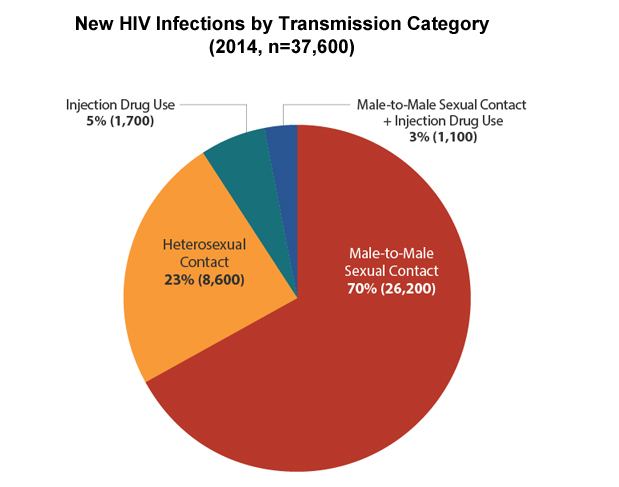
\includegraphics[scale=0.65]{AIDS_sexual.jpg}}	
\end{figure}
\clearpage
\begin{figure}
	\subfigure[Data from CDC]{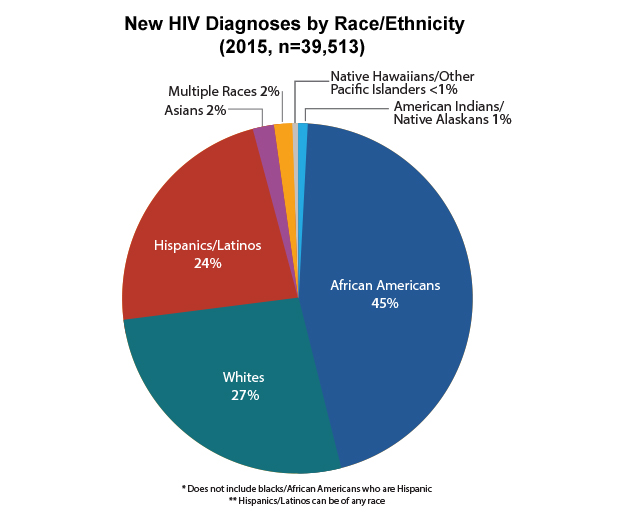
\includegraphics[scale=0.65]{AIDS_ethnic.jpg}}
\end{figure}
Despite scientific progress in medical treatment and countless awareness campaigns, HIV remains a constant and present cause of death. In the United States, in 2014 alone, 6,721 people died from the disease, which was the 8th leading cause of death for individuals aged 25-34, according to the CDC. Worldwide, there were about 1.8 million new cases of HIV in 2016 (most recent available data), with Sub-Saharan Africa accounting for about 64\% of those. There are an estimated 36.7 million individuals living with HIV worldwide, 90\% of whom receive treatment in the form of antiretroviral therapy (ART). Still, of the grand total, about 1 million died in 2016 alone from AIDS-related illnesses.\\

\subsection{Human Immunodeficiency Virus (HIV) - Background on the biology}
HIV is a retrovirus that leads to acquired immune deficiency syndrome, AIDS. Like most of the viruses belonging to the family of \textit{Retroviridae}, HIV only replicates in dividing cells. However, the Human Immunodeficiency Virus has some unique properties even within its family; for instance, it uses the mRNA processing of the cell that invades to synthetize its own viral RNA. Although it had been shown that the dynamics of viral replication is very high \textit{in Vivo} (Ho et al. 1995), the immune system can counteract this replication from 5 to 10 years, depending on the initial infection, sometimes even longer.\\
Infection by the most common variety of the virus, HIV-1, has many complex characteristics that are still not quite completely understood. For instance, the fact that the disease progression can last more than 10 years after the first day of infection; or the fact that immune response only briefly control it, while most viral infections would be eliminated by it. HIV attacks the immune system, primarily infecting CD4-T-cells, a particular class of white blood cells, but also dendritic cells, which play a crucial role in the generation and regulation of adaptive immunity. The T-cell count is normally 500-1500 cells per $\mu$L of blood and, if it drops to 200/$\mu$L or below, then a person is diagnosed with having AIDS. \\
Yet, the CD4 T-cell count is not the only factor used to make a diagnosis on that matter. The Center for Disease Control applies very specific and regularly-updated categories, which include several diseases as symptoms or indicators, that the CDC uses for surveillance purposes. For instance, if a patient with the virus has a T-cell count greater than 500/$\mu$L, but has one of a variety of diseases (from peripheral neuropathy to a recurrent bacteria-pneumonia), then a formal diagnosis is made. The reason for the fall of T-cells is still unknown, but what can be said with confidence is that, because of the central role of CD4 T-cells in immune regulation, their depletion has widespread deleterious effects on the proper functioning of the immune system, which is what causes AIDS to arise.\\
Since the mid-1980's, both stochastic and deterministic models have been developed to describe the immune system in its interaction with HIV. Stochastic models aim to account for the delay of the early events in the disease when there are few infected cells and a small number of particles of the virus. However, because of their applicability to later stages of the evolution of the disease for large populations, most models have been deterministic, as they reflect dynamic changes in mean cell numbers. Deterministic models take into consideration the dynamics of the CD4 cells, latently infected cells and virus populations, as well as the effects of the drug therapy.\\
The dynamics of HIV infection has been incredibly difficult to study, mostly due to ethical reasons (experiments on human are not allowed), so fundamental information to properly modelling the disease has been lacking for years. For instance, it was widely believed that the components of the disease process were slow, as it takes an average of 10 years for the disease to develop. However, mathematical modeling and experiments have shown this to be not exactly the case, as there are different timescales, from minutes to hours to months, in HIV infection. Figure 1.1 shows a typical course of HIV infection. Immediately after the infection the total number of particles of the virus detected in the blood, V, increases rapidly. After a few weeks to months the symptoms disappear and the virus concentration falls to a lower level. Then, an immune response to the virus occurs and antibodies can be detected in the blood. The presence or lack thereof of such antibodies is a critical parameter to determine if a person has been exposed to the virus. A highly defined test is performed to detect these antibodies and, if found, then a person is said to be HIV-positive.

\begin{figure}[H]
	{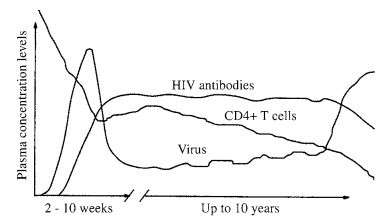
\includegraphics[scale=0.85]{HIV-Infection-Timescale.png}}
	\caption{Schematic time course of a typical HIV infection in an infected adult. The viral concentration, the level of antibodies and the CD4 T-Cells are sketched as a function of time. The early peek represents the primary infection that leads to a period of latency. (From Perelson and Nelson 1999)}
\end{figure}

The level of the virus falls after the initial infection to a level that has been called the set-point. Then, the concentration of the virus seems to remain relatively constant as the CD4 T-cells concentration slowly declines. This period in which the virus concentration is at a quasi-steady state level, while the CD4 T-cells slowly falls, is typically an asymptomatic period, i.e. the person infected does not experience any symptoms that usually would be typical of the disease.\\
Epidemiologists have been puzzled for years about the events that might be happening during the asymptomatic period, until when, in the mid 1990's, became possible to perturb the host-virus system during this period, thanks to the development of new antiretroviral drugs, called protease inhibitors. This drugs block the enzyme protease which HIV uses to  break up large proteins into smaller pieces required to assembly new viral particles. Therefore, in 1994, David Ho, one of the most prominent researchers in the field of HIV treatment, ran an experiment which examined the response of 20 HIV-infected individuals to treatment with ritonavir, a protease inhibitor. The experiment led to dramatic results, with the virus concentration falling rapidly after the ingestion of the drug, as can be seen in figure 1.2.

\begin{figure}[H]
	{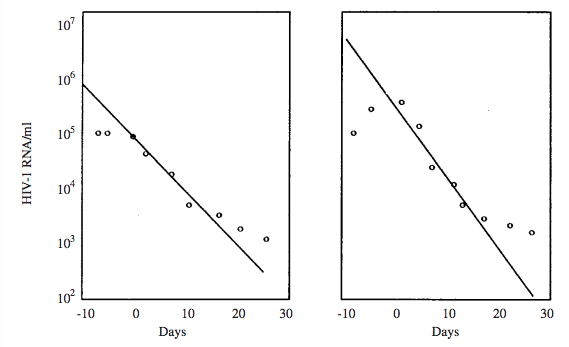
\includegraphics[scale=0.7]{HIV-Protease.png}}
	\caption{After treatment at $t=0$ with ritonavir, the virus concentration declined rapidly. The data are from 2 of the 20 patients studied in Ho et al. (1995), but all 20 patients exhibited similar behavior in the decline of the virus.}
\end{figure}




\chapter{Body}
\section{Modeling HIV Transmission Dynamics - Part I}

\subsection{A first approach}
In modeling epidemics, very often, the population under consideration is assumed to be of fixed size, with births balancing deaths or migration. Such assumption is reasonable when studying endemic diseases over a large period of time and without any disease-induced deaths within the population under study. However, since HIV infections and subsequent development of AIDS have led to increased death rates in various risk groups, the population's demographic structures need to be taken into account in the modeling of the transmission dynamics of the virus.\\
The following model is largely based upon the study conducted by R.M. May and R.M. Anderson titled $\textit{The Transmission Dynamics of the Human Immunodeficiency Virus}$ published in 1988. Such study, despite being understandingly outdated in its approach to the disease (back then there was no treatment for HIV infected, for instance), is nevertheless still regarded as a good pedagogical tool to construct HIV-AIDS models using a flow-chart.\\
Consider a homosexual population of sexually-active males (age 13-65) of varying size $N(t)$ at time $t$. Assume a constant inflow of susceptible individuals at a rate $Q_{1}$ and of HIV-infectives at a rate $Q_{2}$. The population $N(t)$ is then divided in four sub-classes: 
\begin{itemize}
\item Susceptibles $S(t)$, 
\item Infected (also assumed to be infectious) $I(t)$, 
\item pre-AIDS patients $P(t)$,
\item AIDS patients $A(t)$. 
\end{itemize}
The pre-AIDS patients are individuals whose viral count is above 75 copies of virus per milliliter of blood, but have not been diagnosed with having AIDS yet. However, it is assumed that virtually all individuals in the pre-AIDS class will ultimately developed AIDS and therefore join the AIDS class.\\
All subclasses have a natural mortality rate $d$, but the total population $N(t)$ loses individuals at a higher rate from the AIDS class than from any of the others. Susceptibles sexually interact with Infected at a rate $\beta$ and with pre-AIDS patients at a rate $\beta^{\prime}$. As it is assumed that individuals in the pre-AIDS class are less sexually-active than individuals in the Infected class, then $\beta^{\prime} << \beta$. The parameter $c$ indicates the number of sexual partner for unit of time (years, in this case). It is also assumed that a fraction $\epsilon$ of infected individuals will join the pre-AIDS class (depending on the viral count) at a rate $\delta$, while another fraction (1-$\epsilon$) will join the AIDS class directly, at a rate $\delta$, as well.
Individuals in the pre-AIDS class will join the AIDS class at a rate $\alpha_{1}$, which is assumed to be much greater than the natural mortality rate $d$ of the class. Finally, individuals in the AIDS-class will have a disease-induced mortality rate of $\alpha$ and therefore a total mortality rate of ($\alpha$ + $d$). The following transfer diagram provides a helpful visualization of the the aforementioned assumptions.

\begin{center}
	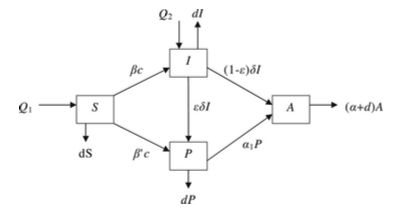
\includegraphics[scale=0.75]{HIV_Flow_Chart.png}
\end{center}

From the assumptions made, we can construct a system of Ordinary Differential Equations to describe the dynamics of the different sub-classes, as follows

\begin{align}
\frac{dS}{dt} = Q_{1} - \left(\frac{\beta cSI}{N} + \frac{\beta^{\prime} cSP}{N}\right) - dS,
\end{align}
\begin{align}
\frac{dI}{dt} = Q_{2} + \frac{\beta cSI}{N} + \frac{\beta^{\prime} cSP}{N} - (\delta + d)I,
\end{align}
\begin{align}
\frac{dP}{dt} = \epsilon\delta I - (\alpha_{1} + d)P,
\end{align}
\begin{align}
\frac{dA}{dt} = (1 - \epsilon)\delta I + \alpha_{1}P - (\alpha + d)A.
\end{align}

We see that we have a system of four differential equations with five variables, as $N(t)$ is not constant. Therefore, using the fact the total population is equal to

$$
N(t) = S(t) + I(t) + P(t) + A(t),
$$
we can rearrange the above system and write it as

\begin{align}
\frac{dN}{dt} = Q_{1} + Q_{2} -dN - \alpha A,
\end{align}
\begin{align}
\frac{dI}{dt} = Q_{2} + \frac{\beta c(N-I-P-A)I}{N} + \frac{\beta^{\prime} c(N-I-P-A)P}{N} - (\delta + d)I,
\end{align}
\begin{align}
\frac{dP}{dt} = \epsilon\delta I - (\alpha_{1} + d)P,
\end{align}
\begin{align}
\frac{dA}{dt} = (1 - \epsilon)\delta I + \alpha_{1}P - (\alpha + d)A,
\end{align}

with $N(0)>0$, $I(0)>0$, $P(0)>0$, $A(0)>0$.\\
Continuity of the right-hand side of the system and its derivative indicates that the model is well-posed for $N>0$. It is also assumed that all variables and parameters be non-negative.\\
Before proceeding in numerical simulations of the model, we first perform some stability analysis of the equilibrium.

\subsection{Equilibrium and Stability Analysis}
In our model we have a constant inflow of infected individuals at a rate $Q_{2}$, therefore the model does not exhibit a diseased-free equilibrium. However, to find all non-negative equilibria of the model, we can solve

$$
Q_{1} + Q_{2} -dN - \alpha A = 0,
$$

$$
Q_{2} + \frac{\beta c(N-I-P-A)I}{N} + \frac{\beta^{\prime} c(N-I-P-A)P}{N} - (\delta + d)I = 0,
$$

$$
\epsilon\delta I - (\alpha_{1} + d)P = 0,
$$

$$
(1 - \epsilon)\delta I + \alpha_{1}P - (\alpha + d)A = 0,
$$

which, as we shall see later, only has one non-negative solution. Such solution is the so-called $\textit{Endemic Equilibrium}$  $E^{\star} = (N^{\star},I^{\star},P^{\star},A^{\star})$, which exists as long HIV infections persist in the population, i.e. $I \neq 0$.\\

On simultaneously solving the above system of algebraic equations, we find

$$
I = \tau \xi \left(\frac{Q_{1} + Q_{2} - d N}{\alpha}\right),
$$

$$
P = \xi \left(\frac{Q_{1} + Q_{2} - d N}{\alpha}\right),
$$

$$
A = \left(\frac{Q_{1} + Q_{2} - dN}{\alpha}\right),
$$

which are all positives for $N<(Q_{1}+Q_{2})/d$.

Here

$$
\tau = \left(\frac{\alpha_{1} + d}{\epsilon \delta}\right),
$$

and

$$
\xi =  \left(\frac{(\alpha + d)}{\alpha_{1} + \frac{(1-\epsilon)}{\epsilon}(\alpha_{1}+d)}\right).
$$

Moreover,
\begin{align*}
Q_{2}N + \xi (\beta c\tau + \beta^{\prime}c) \left[N-(1+\xi+\xi\tau)\left(\frac{Q_{1}+Q_{2}-dN}{\alpha}\right)\right]\left(\frac{Q_{1}+Q_{2}-dN}{\alpha}\right)
\end{align*}
\begin{align*}
- (\delta+d) \xi\tau N \left(\frac{Q_{1}+Q_{2}-dN}{\alpha}\right) = 0.
\end{align*}

To show the existence of the endemic equilibrium $E^{\star}$, we write

\begin{align*}
F(N) = Q_{2}N + \xi (\beta c\tau + \beta^{\prime}c) \left[N-(1+\xi+\xi\tau)\left(\frac{Q_{1}+Q_{2}-dN}{\alpha}\right)\right]\left(\frac{Q_{1}+Q_{2}-dN}{\alpha}\right)
\end{align*}
\begin{align*}
- (\delta+d) \xi\tau N \left(\frac{Q_{1}+Q_{2}-dN}{\alpha}\right).
\end{align*}
From here, it is sufficient to show that the quadratic equation $F(N)$ = 0 has only one non-negative root between 0 and $(Q_{1}+Q_{2})/d$. To prove this, we see that we have

$$
F(0)=  - \xi (\beta c\tau + \beta^{\prime}c) (1+\xi+\xi\tau)\left(\frac{Q_{1}+Q_{2}-dN}{\alpha}\right)^{2} < 0
$$

and

$$
F\left(\frac{Q_{1}+Q_{2}-dN}{d}\right) = Q_{2}\left(\frac{Q_{1}+Q_{2}-dN}{d}\right) > 0.
$$

Also,

$$
F^{\prime}(N) = Q_{2} + \left[(\beta c - (\delta + d))\tau\xi + \beta^{\prime}c + \frac{2\xi d}{\alpha} (1+\tau\xi+\xi)\right] \left(\frac{Q_{1}+Q_{2}-dN}{\alpha}\right)$$
$$
- [\beta c - (\delta + d))\tau\xi + \beta^{\prime}c]\frac{dN}{\alpha}.
$$

From Calculus, we know that if $F^{\prime}(N)>0$ then the equation
$$
F(N) = 0
$$
has exactly one solution, say $N^{\star}$, between 0 and $\left(\frac{Q_{1}+Q_{2}-dN}{d}\right)$. Using $N^{\star}$ then $I^{\star}$, $P^{\star}$, $A^{\star}$ can be found, as well.\\

$\textbf{\emph{Local stability of the equilibrium point}}$\\

We can determine the nature of the local stability of the endemic equilibrium, by finding the characteristic polynomial of the following variational matrix about $E^{\star}$,

\begin{align*}
\begin{bmatrix}
-d & 0 & 0 -\alpha \\
m_{21} & -m_{22} & m_{23} & -m_{24} \\
0 & \epsilon\delta & -(\alpha_{1}+d) & 0 \\
0 & (1-\epsilon)\delta & \alpha_{1} & -(\alpha+d)
\end{bmatrix},
\end{align*}

where

$$
m_{21} = \frac{Q_{2}}{N^{\star}} + [\beta c(\delta+d)]\frac{I^{\star}}{N^{\star}} + \frac{\beta^{\prime}cP^{\star}}{N^{\star}},
$$

$$
m_{22} = \frac{Q_{2}}{I^{\star}} + \frac{\beta cI^{\star}}{N^{\star}} + \frac{\beta^{\prime} cP^{\star}}{N^{\star}} + \frac{\beta c(N^{\star}-I^{\star}-P^{\star}-A^{\star}}{N^{\star})}\left(\frac{\epsilon\delta}{\alpha_{1}+d}\right),
$$

$$
m_{23} = \frac{\beta cI^{\star}}{N^{\star}} + \frac{\beta^{\prime} cP^{\star}}{N^{\star}} + \frac{\beta^{\prime} c(I^{\star}+P^{\star}+A^{\star})}{N^{\star}} - \beta^{\prime}c,
$$

$$
m_{24} = \frac{\beta cI^{\star}}{N^{\star}} + \frac{\beta^{\prime}cP^{\star}}{N^{\star}}.
$$

The characteristic equation equation corresponding to $M(E^{\star})$ is given by
$$
f(\lambda) = \lambda^{4}+ a_{1}\lambda^{3} + a_{2}\lambda^{2} + a_{3}\lambda + a_{4} = 0,
$$
where

$$
a_{1} = 3d + \alpha + \alpha_{1} + m_{22},
$$

$$
a_{2} = (\alpha+d)(\alpha_{1}+d) + d(\alpha+\alpha_{1}+2d+m_{22}) + m_{22}(\alpha+\alpha_{1}+2d) + m_{23}\epsilon\delta+(1-\epsilon)m_{24},
$$

$$
a_{3} = d(\alpha+d)(\alpha_{1}+d) + m_{22}[(\alpha+d)(\alpha_{1}+d) + (\alpha+d)\alpha_{1}+(\alpha_{1}+d)d] + m_{24}[(1-\epsilon)\delta(\alpha_{1}+2d)]$$
$$m_{24}\epsilon\delta\alpha_{1} + m_{23}(\alpha+d)\epsilon\delta + m_{21}(1-\epsilon)\alpha\delta,
$$

$$
a_{4} = m_{22}d(\alpha+d)(\alpha_{1}+d) + m_{23}d(\alpha+d)\epsilon\delta + m_{24}d[\epsilon\delta\alpha_{1} + (1-\epsilon)\delta(\alpha_{1}+d)]$$
$$
+m_{21}\alpha\epsilon\delta\alpha_{1} + m_{21}\alpha(1-\epsilon)\delta(\alpha_{1}+d).
$$

It can readily be seen that $a_{i} > 0 $, where $i=1,2,3,4$, and $a_{1}a_{2}-a_{3}>0$, assuming that $m_{21} >0$, which implies that $\beta c \geq (\delta+d)$. Therefore, the endemic equilibrium $E^{\star}$ is locally asymptotically stable if $a_{3}(a_{1}a_{2}-a_{3}) - a_{1}^{2}a_{4} > 0$.

\subsection{Numerical Analysis and discussion}
To solve the system (2.5)-(2.8) numerically, we use the ode solver $\textit{ode45}$ in MatLab and we also find the endemic equilibrium $E^{\star}$ for the following values of parameters, taken from literature\\

$Q_{1}$=1000, $Q_{2}$=1000, $\epsilon$=0.6; d=0.02, $\alpha$=1, $\alpha_{1}$=0.5, $\beta$=0.15, $\beta^{\prime}$=0.05, c=10, $\delta$=0.4\\

with initial conditions\\
$N(0)=5000, I(0)=2000, P(0)=1000, A(0)=500$.\\
The dynamics of the population was modelled over a time interval of 30 years, following the examples found in the literature.\\

To better see how the constant immigration of both susceptible individuals and of infected people into $N(t)$ affects the dynamics of the population, we also plot our solutions for the system (2.5)-(2.8) if there there was no constant inflow of susceptibles and infected, i.e. $Q_{1}=Q_{2}=0$.

\begin{figure}[H]
	\subfigure[Model with immigration]{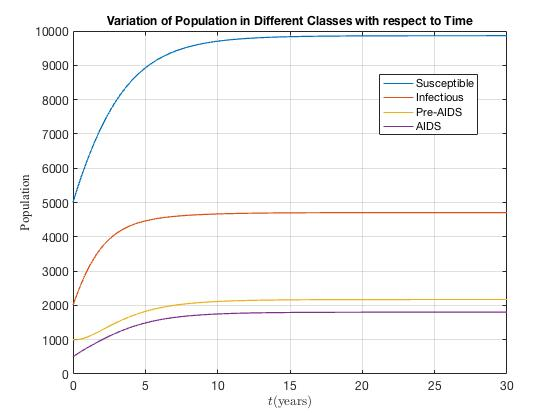
\includegraphics[scale=0.6]{hiv1.jpg}}
\end{figure}
\begin{figure}
	\subfigure[Model without immigration]{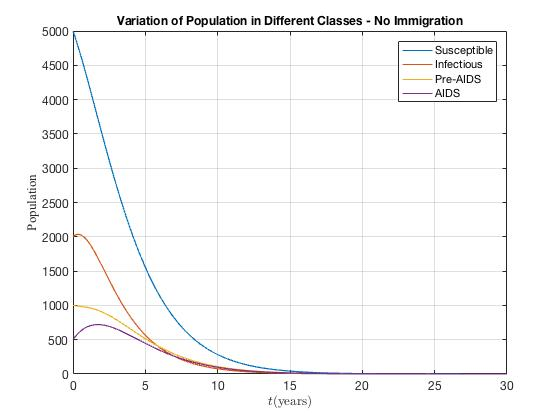
\includegraphics[scale=0.6]{hiv2.jpg}}
	\caption{Visualizing the impact of the inflow of infectious and susceptibles on the dynamics of the population}
\end{figure}

From Figure 2.1a and 2.1b, we can readily see the impact of the constant inflow of susceptible individuals and of infectious (infected) ones on the dynamics of the population.\\
In the case when there is no inflow (Fig.2.1b), the four sub-classes of individuals all decrease, ultimately exhibiting an overall exponential decay, as the total population will approach zero at around $t=15$.\\
As expected, the susceptible population decreases in size at the fastest rate, due to the fact that, without a constant inflow $Q_{1}$, the susceptibles will either die at their natural mortality rate or join either the infectious or the pre-AIDS class that will ultimately die of either AIDS or natural causes. \\
On the other hand, the initial AIDS population actually increases between $t=0$ and around $t=1$. Again, this makes sense, because this sub-class receives an input of infected individuals and pre-AIDS patients, whose total number is initially greater than the number of deaths from the AIDS-class. However, after reaching its maximum at around $t=1$, the AIDS class starts decreasing, with an interflection point at around $t=4$ and then it intersects both the infected and pre-AIDS class at $t=6$ and keeping on decreasing.\\

Conversely, in the case with a constant inflow of both susceptible and infectious individuals (Fig.2.1a), we see that all four subclasses exhibit an initial growth, with both the susceptible class and the infectious class having the faster rate of increase, as expected from the initial conditions $Q_{1}=Q_{2}=1000$. Both classes increase fast at the beginning, then the infectious class starts slowing down its growth around $t=2.5$, while the susceptible class starts to slow down after $t=4$. The infected class reaches its maximum at around $t=10$ then levels off, while the susceptible class reaches its at around $t=12$ and then levels off. \\
On the other hand, the classes of pre-AIDS patients and AIDS-patients grow more slowly compared to $I$ and $N$, increase until around $t=8$, reaching their maximum at around $t=12$ and then level off.\\

$\textbf{\emph{Equilibrium Analysis}}$\\

We focus our equilibrium analysis only to the model with a constant inflow of infected and susceptibles, i.e. $Q_{1}=Q_{2} > 0$. We use the parameters from literature and different sets of initial conditions to show that all the solutions converges to the computed equilibrium. Numerically, we find only one positive equilibrium\\

($N^{\star}$,$I^{\star}$,$P^{\star}$,$A^{\star}$) = (9863,4706,2172,1803),\\

which is the endemic equilibrium $E^{\star}$.
We compute the Jacobian matrix about this equilibrium and we find
\begin{align*}
J(E^{\star}) = \begin{bmatrix}
-0.0200 & 0  & 0  & -1 \\
0.7268  & -1.0660 & -0.7658  & -0.8258 \\
0 & 0.2400  & -0.5200 & 0 \\
0  &  0.1600 & 0.5000  & -1.0200
\end{bmatrix}.
\end{align*}

The eigenvalues are readily found to be
$\lambda_{1}=-0.3436$, $\lambda_{2}=-0.6190 + 0.2824i$, $\lambda_{3}=-0.6190 - 0.2824i$, $\lambda_{4} = -1.0443$.
Thus, we have two real negative eigenvalues and a pair of complex conjugates with negative real parts. Therefore, we have an attractive plane (connected to the real eigenvalues) and an attractive two-dimensional spiral (connected to the complex eigenvalues).\\
From the signs of the real eigenvalues and the signs of the real parts of the complex ones, we can conclude that the endemic equilibrium is locally asymptotically stable. We then plot several solutions with different initial conditions to verify this. The results are shown below.

\begin{figure}[H]
	\subfigure[S vs. P vs. A, 3D]{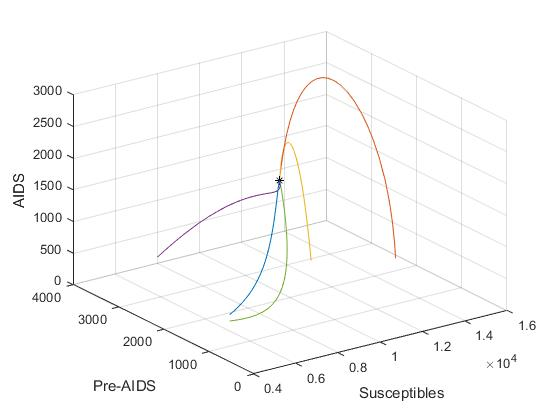
\includegraphics[scale=0.7]{hiv7.jpg}}
	\caption{Visualizing the local stability of the endemic equilibrium $E^{\star}$}
\end{figure}

So, as we can see from Fig2.2, all the solutions tend asymptotically to the endemic equilibrium, as expected from our analysis of the eigenvalues.

\subsection{Final remarks on the model}
All models are wrong, and this one makes no exception.\\
However, the model also provides some insights on how to structure an analysis of HIV transmission dynamics, giving also the opportunity to see how the study of disease was approached in the 1980's, when the epidemic erupted in the US. The model is relatively simple to solve and analyze and it is still regarded as a good pedagogical tool.\\
Nevertheless, it cannot be overstated how not including any medical treatment for HIV, while also limiting the study to a male homosexual population, represents a major flaw of this model, that cannot allow us to apply it to our time. Today we know that HIV is very much heterosexual and that drug treatment can significantly lengthen people's lives, therefore other models are required. \\
We propose one that includes drug therapy in the following section. 

\section{Modeling HIV Transmission Dynamics - Part II}
\subsection{Model of HIV/AIDS with treatment}
Over the course of many years, many treatments for HIV has been tried and implemented. Even though, up until today, there is not an effective cure for this disease, drug treatment has developed incredibly over decades and today individuals with HIV can live long and healthy life, as long as they receive treatment.\\
In fact, the process of HIV-1 pathogenesis can be slowed down by Highly Active Antiretroviral Treatment (HAART). Primarily, HAART inhibits the formation of virus particles, keeping therefore the viral load down and in turn increasing the CD4 cells count.\\
We now provide the description and analysis of a model of HIV transmission dynamics that takes into account treatment. In fact, it also considers the possibility of people receiving alternative treatment(i.e. non-HAART), as it is often the case in regions of the underdeveloped world, where access to Western-medicine-based treatment can be very problematic. The model is largely based on the research work by $\textit{Mukhtar}^{(5)}$.\\

Consider a population of size $N(t)$ at time $t$, divided into five sub-classes:
\begin{itemize}
\item \textit{S}: Susceptibles,
\item \textit{I}: Infected, but not on treatment
\item \textit{H}: Infected and on an alternative (non-HAART) treatment,
\item \textit{J}: Infected and on HAART,
\item \textit{A}: AIDS patients.
\end{itemize}

Therefore the total population $N(t)$ is
$$
N(t) = S(t) + I(t) + H(t) + J(t) + A(t).
$$

We can write down a system of differential equations to describe the population dynamics, as follows
\begin{align}
\frac{dS}{dt} = \mu k - c\beta(I+H+bJ)S - \mu S,
\end{align}
\begin{align}
\frac{dI}{dt} = (1-h)c\beta(I+H+bJ)S - (\mu+k_{1})I + \alpha(1-h_{1})J,
\end{align}
\begin{align}
\frac{dH}{dt} = hc\beta(I+H+bJ)S - (\mu+k_{1}-r)H + ah_{1}J,
\end{align}
\begin{align}
\frac{dJ}{dt} = k_{1}I + (k_{1}-r)H - (\mu+k_{2}+\alpha)J,
\end{align}
\begin{align}
\frac{dA}{dt} = k_{2}J - (\mu+d)A.
\end{align}

We now proceed to explain the parameters that appear in the above system
\begin{itemize}
\item $\mu$ is the natural mortality rate,
\item $k$ is the recruitment rate of the population,
\item $\alpha$ is the antiretroviral therapy rate,
\item $c$ is the average number of contacts between individuals per unit of time,
\item $\beta$ and b$\beta$ are the probabilities of diseased transmission per contact by an infective $I$ and by an infective $J$ respectively,
\item $k_{1}$ is the transfer rate from the asymptomatic stage to the symptomatic stage,
\item $r$ relates to the retardation effect of non-antiretroviral treatment,
\item $k_{2}$ is the transfer rate from the class $J$ to the class $A$,
\item $h$ is the fraction of the infected individuals that moves to non antiretroviral (non-ARV ) treatment,
\item $h_{1}$ is the fraction of infected individuals that have previously received ARV-treatment but now move to non-ARV treatment,
\item $d$ is the disease-induced death rate.
\end{itemize}

The variable $A$ (AIDS patients) only appears in equation (2.13) of the system (2.9)-(2.13), which means there is no interaction between the people of this class and the other four classes. That is because AIDS patients are assumed to be extremely weaken by the disease and therefore sexually inactive, so that they cannot infect others.\\
Thus, the $S$, $I$, $H$ and $J$ classes are assumed to be the active classes. The term $(I+H+bJ)S$ in equation (2.9)-(2.11) is known as an $\textit{interaction term}$. This term carries all four active classes and reflects the frequency of contact between susceptible and infected individuals.\\
For the following analysis, we can suppress equation (2.13) and our new system becomes

\begin{align}
\frac{dS}{dt} = \mu k - c\beta(I+H+bJ)S - \mu S,
\end{align}
\begin{align}
\frac{dI}{dt} = (1-h)c\beta(I+H+bJ)S - (\mu+k_{1})I + \alpha(1-h_{1})J,
\end{align}
\begin{align}
\frac{dH}{dt} = hc\beta(I+H+bJ)S - (\mu+k_{1}-r)H + ah_{1}J,
\end{align}
\begin{align}
\frac{dJ}{dt} = k_{1}I + (k_{1}-r)H - (\mu+k_{2}+\alpha)J.
\end{align}

\subsection{Equilibria and Stability}
To find the equilibria of the model (2.14)-(2.17) we have to solve

$$
\mu k - c\beta(I+H+bJ)S - \mu S = 0,
$$

$$
(1-h)c\beta(I+H+bJ)S - (\mu+k_{1})I + \alpha(1-h_{1})J = 0,
$$

$$
hc\beta(I+H+bJ)S - (\mu+k_{1}-r)H + \alpha h_{1}J = 0,
$$

$$
k_{1}I + (k_{1}-r)H - (\mu+k_{2}+\alpha)J = 0,
$$

which yields two critical points (equilibria). The first is found to be 

$$
(S_{0},I_{0},H_{0},J_{0}) = (k,0,0,0),
$$

which is the trivial critical point (disease-free equilibrium), and we indicate it as $E_{0}$. The second one is given by
\clearpage
\begin{align}
S_{1} = \frac{\mu+k_{1})\xi_{1} - \mu\alpha(1-h_{1})r}{c\beta[\xi_{3}+hr(\mu+k_{2}-b\mu)+\alpha h_{1}r]},
\end{align}

\begin{align}
I_{1} = \frac{\mu k [(1-h)\xi_{1} + (k_{1}-r)\alpha(1-h_{1})]}{(\mu+k_{1})\xi_{1} - \mu\alpha(1-h_{1})r},
\end{align}

\begin{align}
H_{1} = \frac{\mu k[h\xi_{2}+k_{1}\alpha h_{1}]}{(\mu+k_{1})\xi_{1} - \mu\alpha(1-h_{1})r},
\end{align}

\begin{align}
J_{1} = \frac{\mu k[(\mu+k_{1}-r)k_{1} - h\mu r]}{(\mu+k_{1})\xi_{1} - \mu\alpha(1-h_{1})r},
\end{align}

which is the endemic equilibrium ($E_{1}$), where

\begin{align*}
\xi_{1} = (\mu+k_{1}-r)(\mu + k_{2} +\alpha) - \alpha(k_{1}-r),
\end{align*}
\begin{align*}
\xi_{2} = (\mu+k_{1})(\mu+k_{2}+\alpha)-\alpha k_{1},
\end{align*}
\begin{align*}
\xi_{3} = (\mu+k_{1}-r)(\mu+k_{2}+\alpha+bk_{1}).
\end{align*}

To study the nature of the equilibria we first need to compute the $\textit{basic reproduction number}$ $R_{0}$, which is defined as the expected number of secondary infections arising from a single individual during his/her infectious period, in a population of susceptibles. This parameter plays an important role in the control and eradication of epidemics. \\
If $R_{0}<1$, then, on average, an infected individual produces less than one newly infected individual and the epidemic dies out. On the other hand, if $R_{0} >1$, then each infected individual produces, on average, more than one newly infected individual and, therefore, the epidemic spreads out into the population. In such regard, $R_{0}$ is often considered the threshold quantity that indicates if an infection will invade and persist a population. 
For the system (2.14)-(2.17) the basic reproduction number is found to be

\begin{align}
R_{0} = \frac{c\beta k[\xi_{3}+hr(\mu+k_{?}-b\mu)+\alpha h_{1}r]}{(\mu+k_{1})\xi_{1} -\mu\alpha(1-h_{1})r}.
\end{align}
From literature, we know that the disease-free equilibrium $E_{0}$ is locally asymptotically stable if $R_{0} < 1$ and unstable otherwise. Whereas, the endemic equilibrium $E_{1}$ is stable if $R_{0} > 1$ and unstable if $R_{0} < 1$.\\
In the following section we perform some numerical analysis with different values of parameters to simulate both the case when $R_{0} < 1$ and $R_{0}>1$.

\section{Numerical Simulations}
For the first simulation we use the following variables for the parameters, taken from literature
\\

$k$=120, $\beta$=0.000035, $b$ = 0.3, $\mu$=0.02, $c$=3, $k_{1}$=0.01, $k_{2}$=0.02 $\alpha$=0.01, $h$=0.01, $r$=0.001 and $h$=0.02.\\

By plugging in those values into (2.22) we obtain
$$
R_{0} = 0.45 < 1,
$$
which means that the epidemic should die out for the given values of the parameters. We now plot our results

\begin{figure}[H]
	{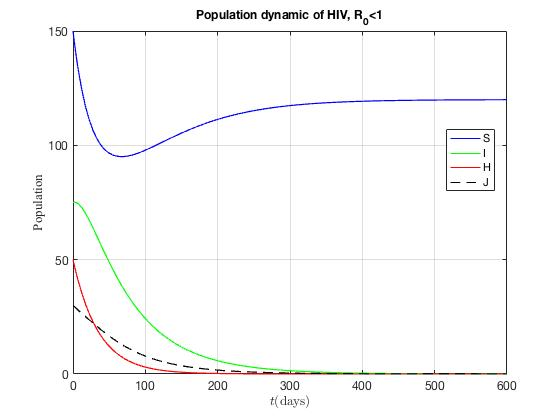
\includegraphics[scale=0.7]{hiv_art.jpg}}
	\caption{Simulation for $R_{0} < 1$}
\end{figure}

Thus, we see from figure 2.3 that, for a basic reproduction number that is less than unity, the population of susceptibles $S$ decreases at first and then starts increasing back at around $t=95$ as the infected population of all the other classes, regardless of treatment, starts to quickly approaching zero. The susceptible population seems to be levelling off at around $t=400$, when the classes $I$, $J$ and $H$ all reaches zero.\\
From an equilibrium point perspective, this makes sense as we have a value for $R_{0}$ that is less then 1; therefore, the solutions will tend to the locally asymptotically stable disease-free equilibrium, and the disease will eventually die out.\\

Now we simulate the case for which the basic reproduction number is greater than unity. For this numerical simulation we use the parameters (from literature)\\

$k$=120, $\beta$=0.0005, $b$ = 0.3, $\mu$=0.02, $c$=3, $k_{1}$=0.01, $k_{2}$=0.02 $\alpha$=0.01, $h$=0.01, $r$=0.001 and $h$=0.02.\\

Plugging those values back into (2.22) yields

$$
R_{0} = 3.8 > 1,
$$
which means that the epidemic should invade the population and persist. We now plot our results

\begin{figure}[H]
	{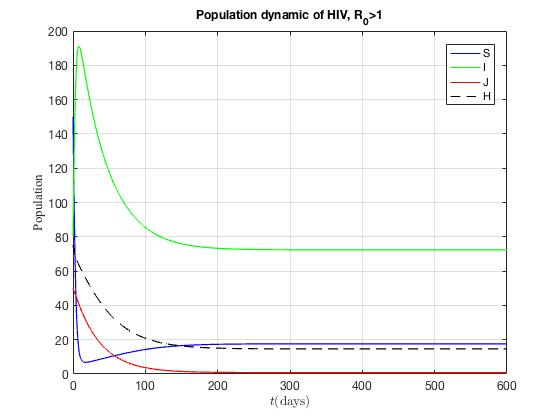
\includegraphics[scale=0.7]{hiv_art2.jpg}}
	\caption{Simulation for $R_{0} > 1$}
\end{figure}

Thus, we see that the class of susceptible individuals $S$ rapidly decreases up until $t=20$ when it reaches its minimum, then starts increasing asymptotically towards the endemic equilibrium as time goes on. On the other hand, the class of infected individuals with no treatment $I$, rapidly increases at the beginning, almost mirroring the class $S$, up until around $t=20$ when it reaches its maximum then starts to decrease until around $t=200$, when it levels off. The classes of infected with ARV treatment $J$ and infected with no ARV treatment $H$ exhibit an exponential decay from the beginning.\\
This is in accordance with the expected behavior from our equilibrium analysis, as we see that for a basic reproduction number $R_{0}$ greater than unity, the disease spreads into the population and all solution tend asymptotically to the endemic equilibrium.

\subsection{Final remarks on the model}
So we have seen that this model takes into account antiretroviral treatment as long as alternative forms of treatments in the modeling of the dynamics of a population. In this regard, it represents a step forward compared to the model analysed in section 2.1.1, but it can readily be seen how this model has built upon some of the insights provided by the earlier model.\\
Moreover, including the possibility of no-ARV treatment is an extremely realistic feature to be added to the model, as many individuals across the world, especially in underdeveloped countries, do not have access to Western-medicine-based treatments.

\chapter{Conclusion}
In this paper we have covered only a few aspects that have to be considered when modeling HIV-AIDS epidemic and we focused our analysis on the transmission dynamics of the virus within a certain population.\\
We have briefly explored the evolution of epidemic models and seen how they have changed over time, being able to adapt to the newest and up-to-date scientific knowledge. HIV is still very much an epidemic today as it was in the 1980's, with as many as 36 million people living with AIDS worldwide. Fortunately, in the last 30 years significant progress has been made in the treatment of HIV, even though an effective cure is yet to be found.\\
Implementing good models able to accurately predict the dynamics of HIV is critically important for the development of new and more effective treatments, as well as instituting comprehensive programs to narrow the risks of a spread of the disease.\\
As HAART medication still remains often not accessible to many people around the world, it is perhaps necessary to use different strategies to contain the risks of HIV transmission, such as awareness campaigns to educate men, women and young people about the dangers connected to the disease and how to protect themselves from it.\\ 


\chapter{References}
\begin{thebibliography}{9}
	\bibitem{anderson} 
	Anderson, R.M. and May, R.M. 
	\textit{The Transmission Dynamics of the Human Immunodeficiency Virus}.
	Philosophical Transactions of the Royal Society of London. Series B, Biological Sciences. Vol.321, No.1207, Oct 31, 1988
	\bibitem{center} 
	Center for Disease Control (CDC)
	\textit{Current Trends Update on Acquired Immune Deficiency Syndrome (AIDS) - United States}.
	MMWR 31(37):507-508
	\bibitem{li} 
	Li Wu, Vineet N. Kawalramani 
	\textit{Dendritic-cells interaction with HIV: infection and viral dissemination}.
	Nat Rev Immunol. 2006 Nov; 6(11): 859-868.
	\bibitem{mann} 
	Mann, J.M.
	\textit{AIDS: A worldwide pandemic}.
	In Current Topics in AIDS Volume 2, edited by Gottlieb, M.S. et al. John Wiley \& Sons, 1989
	\bibitem{mukhtar} 
	Mukhtar, Abdulaziz Y.A.
	\textit{Mathematical Modeling of population dynamics of HIV with antiretroviral treatment ad herbal medicine}.
	February 2014
	\bibitem{murray} 
	Murray, J.D. 
	\textit{Mathematical Biology: An Introduction}.
	Springer, New York, 2004.
	\bibitem{naresh} 
	Naresh R., Tripathi A., Sharma D.
	\textit{Modeling and analysis of the spreads of AIDS epidemic with immigration of HIV infectives}.
	Mathematical and Computer Modeling, Elsevier, 2008
	\bibitem{perelson} 
	Perelson, a.s., \& Nelson, P.W.
	\textit{Mathematical Analysis of HIV-1 Dynamics in Vivo}.
	1999
	\bibitem{the} 
	The New York Times
	\textit{Magic Johnson End His Career, Saying He Has AIDS Infection}.
	November 8th, 1991
	\bibitem{the} 
	The Guardian
	\textit{Death of rock star makes AIDS real}.
	November 26th, 1991
	\bibitem{unaids} 
	UNAIDS
	\textit{Global Report 2013}.
	2013

\end{thebibliography}

\chapter{Appendix}
\section{Matlab Code}
\subsection{Code Implemented for Section 2.1.3}
\lstinputlisting{hiv3.m}
\
\lstinputlisting{hiv4.m}
\clearpage
\lstinputlisting{hiv3_plot.m}
\clearpage
\subsection{Code Implemented for Section 2.3}
\lstinputlisting{Delay_Mahaffy1b.m}
\clearpage
\lstinputlisting{hiv_art.m}
\
\lstinputlisting{hiv_art_plot.m}
\clearpage
\lstinputlisting{hiv_art2.m}
\
\lstinputlisting{hiv_art2_plot.m}

%chapter{Problem 6}
%From Problem 5b, we have
$$
E(t) = \sum_{j=0}^{\infty} (N_{0}+j)P_{N_{0}+j}(t) = N_{0}e^{\lambda t}
$$
We have $N_{0}=10,000$ and that the total number of births occurred in 20 days is 4,500.\\
So, assuming that no deaths will occur in this period since this is a birth-only stochastics process, we have that our expected population at $t=20$ is
$$
E(20) = 4,500 + 10,000 = 14,500.
$$
Therefore
$$
14,500 = 10,000e^{\lambda 20},
$$
from which we can easily solve for $\lambda$
$$
\lambda = \frac{\ln \left(\frac{14,500}{10,000}\right)}{20}
$$
from which we obtain
$$
\lambda \approx 0.0186
$$
Therefore the population has a growth rate of 1.86\%.

%\chapter{Problem 3}
%\input{Problem3_Latex}

%\chapter{Computational Application}
%\input{chapter4}





\end{document}
